\documentclass[11pt,a4paper]{article}

\usepackage[utf8]{inputenc}
\usepackage[T1]{fontenc}
\usepackage{lmodern}
\usepackage[margin=0.72in]{geometry}
\usepackage[table]{xcolor}
\usepackage{array}
\usepackage{tabularx}
\usepackage{booktabs}
\usepackage{enumitem}
\usepackage{titlesec}
\usepackage{fancyhdr}
\usepackage{lastpage}
\usepackage{hyperref}
\usepackage{tikz}

\definecolor{TextInk}{HTML}{233142}
\definecolor{HeadingBlue}{HTML}{1D3557}
\definecolor{AccentTeal}{HTML}{2A7F92}
\definecolor{AccentGold}{HTML}{C58B4E}
\definecolor{AccentRed}{HTML}{B85C5A}
\definecolor{RuleGray}{HTML}{D6E0E5}
\definecolor{TableStripe}{HTML}{F3F8FA}
\definecolor{SoftBlue}{HTML}{EEF6F8}
\definecolor{SoftRed}{HTML}{FBF0EF}

\hypersetup{
  colorlinks=true,
  linkcolor=HeadingBlue,
  urlcolor=AccentTeal,
  pdftitle={IB Geography SL Paper 1 Full Simulation Set 3 - 2026-05-07},
  pdfauthor={IB Geography SL Preparation}
}

\color{TextInk}
\setlength{\parskip}{0.45em}
\setlength{\parindent}{0pt}
\setlength{\tabcolsep}{5pt}
\renewcommand{\arraystretch}{1.16}
\setlist[enumerate]{leftmargin=1.55em,itemsep=5pt,topsep=5pt}

\newcolumntype{Y}{>{\raggedright\arraybackslash}X}
\newcolumntype{L}[1]{>{\raggedright\arraybackslash}p{#1}}
\newcolumntype{C}[1]{>{\centering\arraybackslash}p{#1}}

\titleformat{\section}
  {\normalfont\huge\sffamily\bfseries\color{HeadingBlue}}
  {}{0pt}{}
  [\vspace{0.12em}{\color{AccentGold}\titlerule[1pt]}]
\titleformat{\subsection}
  {\normalfont\Large\sffamily\bfseries\color{AccentTeal}}
  {}{0pt}{}
\titleformat{\subsubsection}
  {\normalfont\large\sffamily\bfseries\color{HeadingBlue}}
  {}{0pt}{}

\pagestyle{fancy}
\setlength{\headheight}{14pt}
\fancyhf{}
\fancyhead[L]{\sffamily\color{AccentTeal}Set 3}
\fancyhead[R]{\sffamily\color{HeadingBlue}Paper 1 Simulation}
\fancyfoot[C]{\sffamily\color{HeadingBlue}\thepage\ of \pageref{LastPage}}
\renewcommand{\headrulewidth}{0.4pt}

\newcommand{\term}[1]{\textcolor{HeadingBlue}{\textbf{#1}}}
\newcommand{\exam}[1]{\textcolor{AccentTeal}{\textbf{#1}}}
\newcommand{\markpts}[1]{\hfill\textbf{[#1]}}
\newcommand{\boxnote}[3]{%
\noindent\colorbox{#1}{%
  \begin{minipage}{0.965\textwidth}
  \sffamily
  \textbf{\textcolor{HeadingBlue}{#2}} #3
  \end{minipage}
}}

\begin{document}

\begin{center}
  {\sffamily\bfseries\color{HeadingBlue}\LARGE IB Geography SL}\\[0.2em]
  {\sffamily\bfseries\color{AccentTeal}\Large Paper 1 Full Simulation: Set 3}\\[0.3em]
  {\sffamily\color{TextInk}Thursday 2026-05-07: Urban Environments + Food And Health}
\end{center}

\boxnote{SoftRed}{Practice-paper notice.}{This is an IB-style practice paper
created for revision. It is not an official IB past paper or official IB mark
scheme. Complete it without notes before using the marking guide.}

\section{Instructions}

\begin{tabularx}{\textwidth}{L{0.25\textwidth}Y}
\toprule
\textbf{Total time} & \term{1 hour 30 minutes}. Spend about \term{45 minutes}
on each option. \\
\textbf{Total marks} & \term{40 marks}. Each option is worth \term{20 marks}. \\
\textbf{Structure} & Answer every structured question. For each option, choose
\term{one} of the two 10-mark extended-answer prompts. \\
\bottomrule
\end{tabularx}

\newpage

\section{Option G: Urban Environments}

\subsection{Source A: Uneven Regeneration In A Post-Industrial City}

Source A shows selected outcomes for four areas of a post-industrial city after
several years of regeneration policy. The data are illustrative.

\rowcolors{2}{TableStripe}{white}
\begin{tabularx}{\textwidth}{L{0.24\textwidth}C{0.15\textwidth}C{0.15\textwidth}C{0.15\textwidth}Y}
\toprule
\textbf{Area} & \textbf{Property-value change} & \textbf{Affordable homes per
1000 residents} & \textbf{Jobs within 30 min by transit} & \textbf{Main outcome} \\
\midrule
Waterfront redevelopment zone & +64\% & 14 & 76\% & New offices and
high-income housing \\
Central business district & +31\% & 9 & 89\% & More jobs and services, but
high land values \\
Inner neighbourhood & +12\% & 36 & 44\% & Some improvements, but service gaps
remain \\
Vacant industrial fringe & -4\% & 20 & 23\% & Derelict land and weak access \\
\bottomrule
\end{tabularx}
\rowcolors{2}{}{}

\subsubsection{Visual Source A}

Longer bars show higher values. Property-value change is shown as a positive
or negative percentage.

\begin{center}
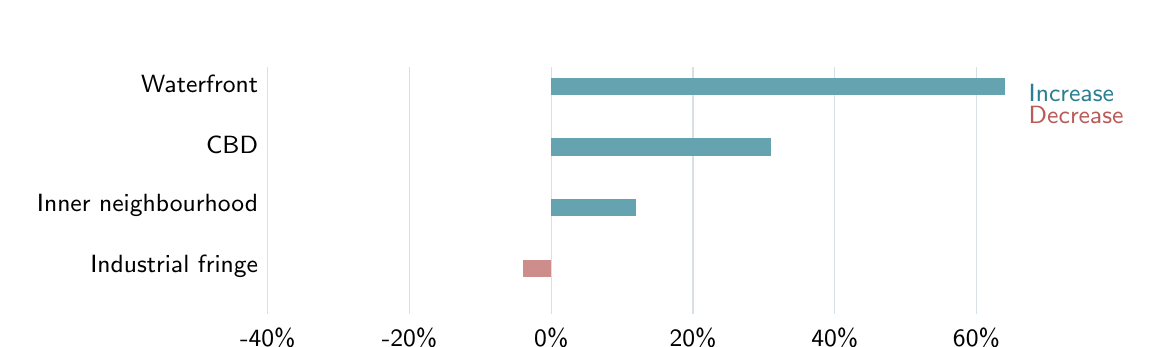
\begin{tikzpicture}[x=0.09cm,y=0.55cm, every node/.style={font=\sffamily\small}]
  \draw[RuleGray] (40,0.9) -- (40,6.6);
  \foreach \x/\lab in {0/-40,20/-20,40/0,60/20,80/40,100/60} {
    \draw[RuleGray] (\x,0.9) -- (\x,6.6);
    \node[anchor=north] at (\x,0.8) {\lab\%};
  }
  \node[anchor=east] at (0,6.2) {Waterfront};
  \draw[fill=AccentTeal!72, draw=none] (40,5.95) rectangle (104,6.35);
  \node[anchor=east] at (0,4.8) {CBD};
  \draw[fill=AccentTeal!72, draw=none] (40,4.55) rectangle (71,4.95);
  \node[anchor=east] at (0,3.4) {Inner neighbourhood};
  \draw[fill=AccentTeal!72, draw=none] (40,3.15) rectangle (52,3.55);
  \node[anchor=east] at (0,2.0) {Industrial fringe};
  \draw[fill=AccentRed!70, draw=none] (36,1.75) rectangle (40,2.15);
  \node[anchor=west, color=AccentTeal] at (106,6.0) {Increase};
  \node[anchor=west, color=AccentRed] at (106,5.5) {Decrease};
\end{tikzpicture}
\end{center}

\subsection{Questions}

Answer all parts. For Question 4, answer either \term{4(a)} or \term{4(b)}.

\begin{enumerate}
  \item \exam{State} two pieces of evidence from Source A that show the
  benefits of regeneration are uneven. \markpts{2}

  \item \exam{Describe} two contrasts between the waterfront redevelopment zone
  and the vacant industrial fringe. \markpts{4}

  \item \exam{Explain} two reasons why urban regeneration can create winners
  and losers. \markpts{4}

  \item Answer either 4(a) or 4(b). \markpts{10}
  \begin{enumerate}[label=\textbf{\alph*.},leftmargin=1.6em]
    \item Using one or more named examples, \exam{examine} the social and
    economic impacts of gentrification.

    \item Using one named city, \exam{evaluate} strategies used to manage urban
    decline or deprivation sustainably.
  \end{enumerate}
\end{enumerate}

\newpage

\section{Option F: Food And Health}

\subsection{Source B: Stakeholders, Food Security, And Health}

Source B compares possible effects of four stakeholder actions. Scores run from
1 to 5, where 5 is strongest. The data are illustrative.

\rowcolors{2}{TableStripe}{white}
\begin{tabularx}{\textwidth}{L{0.21\textwidth}C{0.11\textwidth}C{0.11\textwidth}C{0.11\textwidth}C{0.11\textwidth}Y}
\toprule
\textbf{Stakeholder action} & \textbf{Food availability} & \textbf{Diet quality}
& \textbf{Equity reach} & \textbf{Sust.} & \textbf{Main limitation} \\
\midrule
Government school meals & 4 & 4 & 5 & 3 & Funding and coverage may be uneven \\
TNC convenience-food expansion & 5 & 1 & 3 & 2 & Ultra-processed diets and
market power \\
Smallholder co-operative & 3 & 4 & 3 & 4 & Limited finance and scale \\
NGO WASH and vaccination programme & 1 & 2 & 4 & 3 & Does not directly
increase food supply \\
\bottomrule
\end{tabularx}
\rowcolors{2}{}{}

\subsubsection{Visual Source B}

Longer bars show stronger scores.

\begin{center}
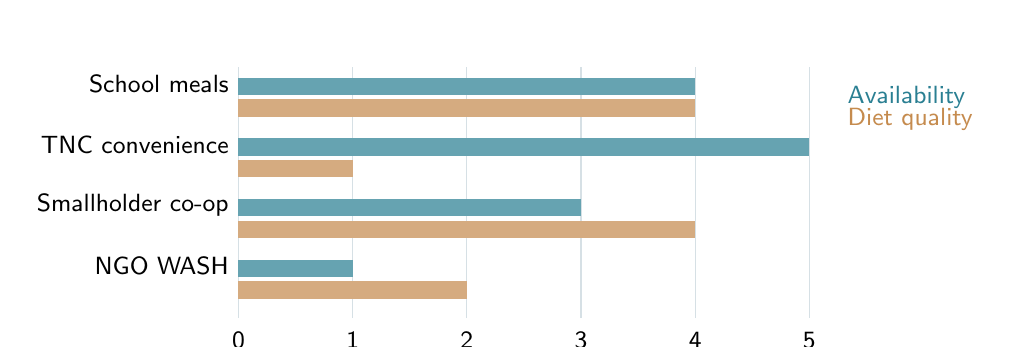
\begin{tikzpicture}[x=1.45cm,y=0.55cm, every node/.style={font=\sffamily\small}]
  \foreach \x in {0,1,2,3,4,5} {
    \draw[RuleGray] (\x,0.8) -- (\x,6.6);
    \node[anchor=north] at (\x,0.7) {\x};
  }
  \node[anchor=east] at (0,6.2) {School meals};
  \draw[fill=AccentTeal!72, draw=none] (0,5.95) rectangle (4,6.35);
  \draw[fill=AccentGold!72, draw=none] (0,5.45) rectangle (4,5.85);
  \node[anchor=east] at (0,4.8) {TNC convenience};
  \draw[fill=AccentTeal!72, draw=none] (0,4.55) rectangle (5,4.95);
  \draw[fill=AccentGold!72, draw=none] (0,4.05) rectangle (1,4.45);
  \node[anchor=east] at (0,3.4) {Smallholder co-op};
  \draw[fill=AccentTeal!72, draw=none] (0,3.15) rectangle (3,3.55);
  \draw[fill=AccentGold!72, draw=none] (0,2.65) rectangle (4,3.05);
  \node[anchor=east] at (0,2.0) {NGO WASH};
  \draw[fill=AccentTeal!72, draw=none] (0,1.75) rectangle (1,2.15);
  \draw[fill=AccentGold!72, draw=none] (0,1.25) rectangle (2,1.65);
  \node[anchor=west, color=AccentTeal] at (5.25,5.9) {Availability};
  \node[anchor=west, color=AccentGold] at (5.25,5.4) {Diet quality};
\end{tikzpicture}
\end{center}

\subsection{Questions}

Answer all parts. For Question 4, answer either \term{4(a)} or \term{4(b)}.

\begin{enumerate}
  \item \exam{State} two stakeholder contrasts shown in Source B. \markpts{2}

  \item \exam{Describe} two ways Source B suggests stakeholder actions can
  produce mixed food and health outcomes. \markpts{4}

  \item \exam{Explain} two ways stakeholders can reduce health inequality.
  \markpts{4}

  \item Answer either 4(a) or 4(b). \markpts{10}
  \begin{enumerate}[label=\textbf{\alph*.},leftmargin=1.6em]
    \item Using one named example, \exam{to what extent} do transnational
    corporations improve food security and health?

    \item Using one or more named examples, \exam{evaluate} the role of
    governments, NGOs, or local communities in reducing food and health
    inequalities.
  \end{enumerate}
\end{enumerate}

\end{document}
